% only the text for the summary

\newpage
\setcounter{page}{1}
\pagenumbering{arabic}

\newcommand{\summaryintrosmallspace}{0.05cm}
\newcommand{\summaryintrobigspace}{0.3cm}

\begin{figure}
	\centering
	\minipage{0.25\textwidth}
	
\includegraphics[width=\linewidth]{images/logo/logo_without_name.png}
	\endminipage\hfill
	\minipage{0.70\textwidth}
	\textbf{Politecnico di Torino} \vspace{\summaryintrosmallspace} \\
	Master Thesis in Computer Engineering \vspace{\summaryintrosmallspace} \\
	Graduation Session: October 2025 \vspace{\summaryintrobigspace} \\
	\textbf{Particle Tracking Acceleration} \vspace{\summaryintrobigspace} \\
	\textbf{Supervisor:} Riccardo Cantoro\vspace{\summaryintrosmallspace} \\
	\textbf{Company Tutor:} Kamel Abdelouahab \vspace{\summaryintrosmallspace} \\
	\textbf{Candidate:} Francesco Risso
	\endminipage
\end{figure}

\newcommand{\summarysection}[1]{\vspace{-.25cm}\section*{#1}\vspace{-.25cm}}

\summarysection{Introduction}

For the better understanding of what happens during a visual experiment, the possibility of recording the experiment itself and watching it again at a later time is crucial.
%For having a better understanding what happens during an experiment, and extracting as much information as possible from it, the possibility of recording the experiment itself and watching it again at a later time is crucial.
While for many cases achieving this is just a matter of recording the event with a camera, some complex situations require more attention.
One such case is when the nature of the experiments requires to understand 3D data, where a 2D video would not carry the necessary information.

% Recording 3D data is a complex task, since cameras work by projecting the real world onto a 2D sensor.
% Still, having ``3D footage'' it is quite useful to better understand the world that surrounds us.
This thesis tackles the task of reconstructing the 3D trajectory of small bubbles moving in the air, observed by a setup of 3 or 4 cameras.
The experiment aims to better understand and describe the movement of the air that surrounds us, which emerged as a key factor in understanding the transmission of COVID-19.
The expected solution should maximize the reconstruction quality, while always keeping the processing time under control, to have a real-time processing on the captured images.

\summarysection{Solution overview}

As commonly done in literature, the final solution splits the task into a 4-step pipeline.
Each step is computed in parallel by a separate process, which communicates with the others by means of a shared memory.
The captured video traverses therefore the following transformation steps:
\begin{itemize}
	\itemsep 0em
	\item \textbf{Locate}: within a single frame, extract the 2D coordinates of the bubbles;
	\item \textbf{3D matching}: combine information of the different cameras to reconstruct the 3D positions;
	\item \textbf{Linking}: join together bubbles from consecutive timestamps into \textbf{tracklets};
	\item \textbf{Visualization}: display the tracklets on a 2D screen, in an intuitive way.
\end{itemize}

\summarysection{Locate}

For the \textit{Locate} step, we used a real experiment to benchmark the multiple approaches available in literature, as well as new algorithms invented within this thesis (the ones marked by * in figure~\ref{fig:intro:locate-speed}).
The most important metric was the speed, since the algorithm has to process the frames in real-time.
On top of that, quality was evaluated by checking the percentage of bubbles that were missed.
Figure~\ref{fig:intro:locate-speed} compares the different speeds of the approaches with the target speed ($3~\textnormal{cameras} \cdot 30~\sfrac{\textnormal{FPS}}{\textnormal{camera}} = 90~\textnormal{FPS}$): while it may seem that none of them reaches the target, a clean-sheet implementation of the best one managed to reach the target speed.
The final choice for the \textit{Locate} step is a new algorithm that includes a CPU portion to find the bubbles, and a GPU section to simultaneously find the coordinates of all bubble centroids.

\begin{figure}
	\centerline{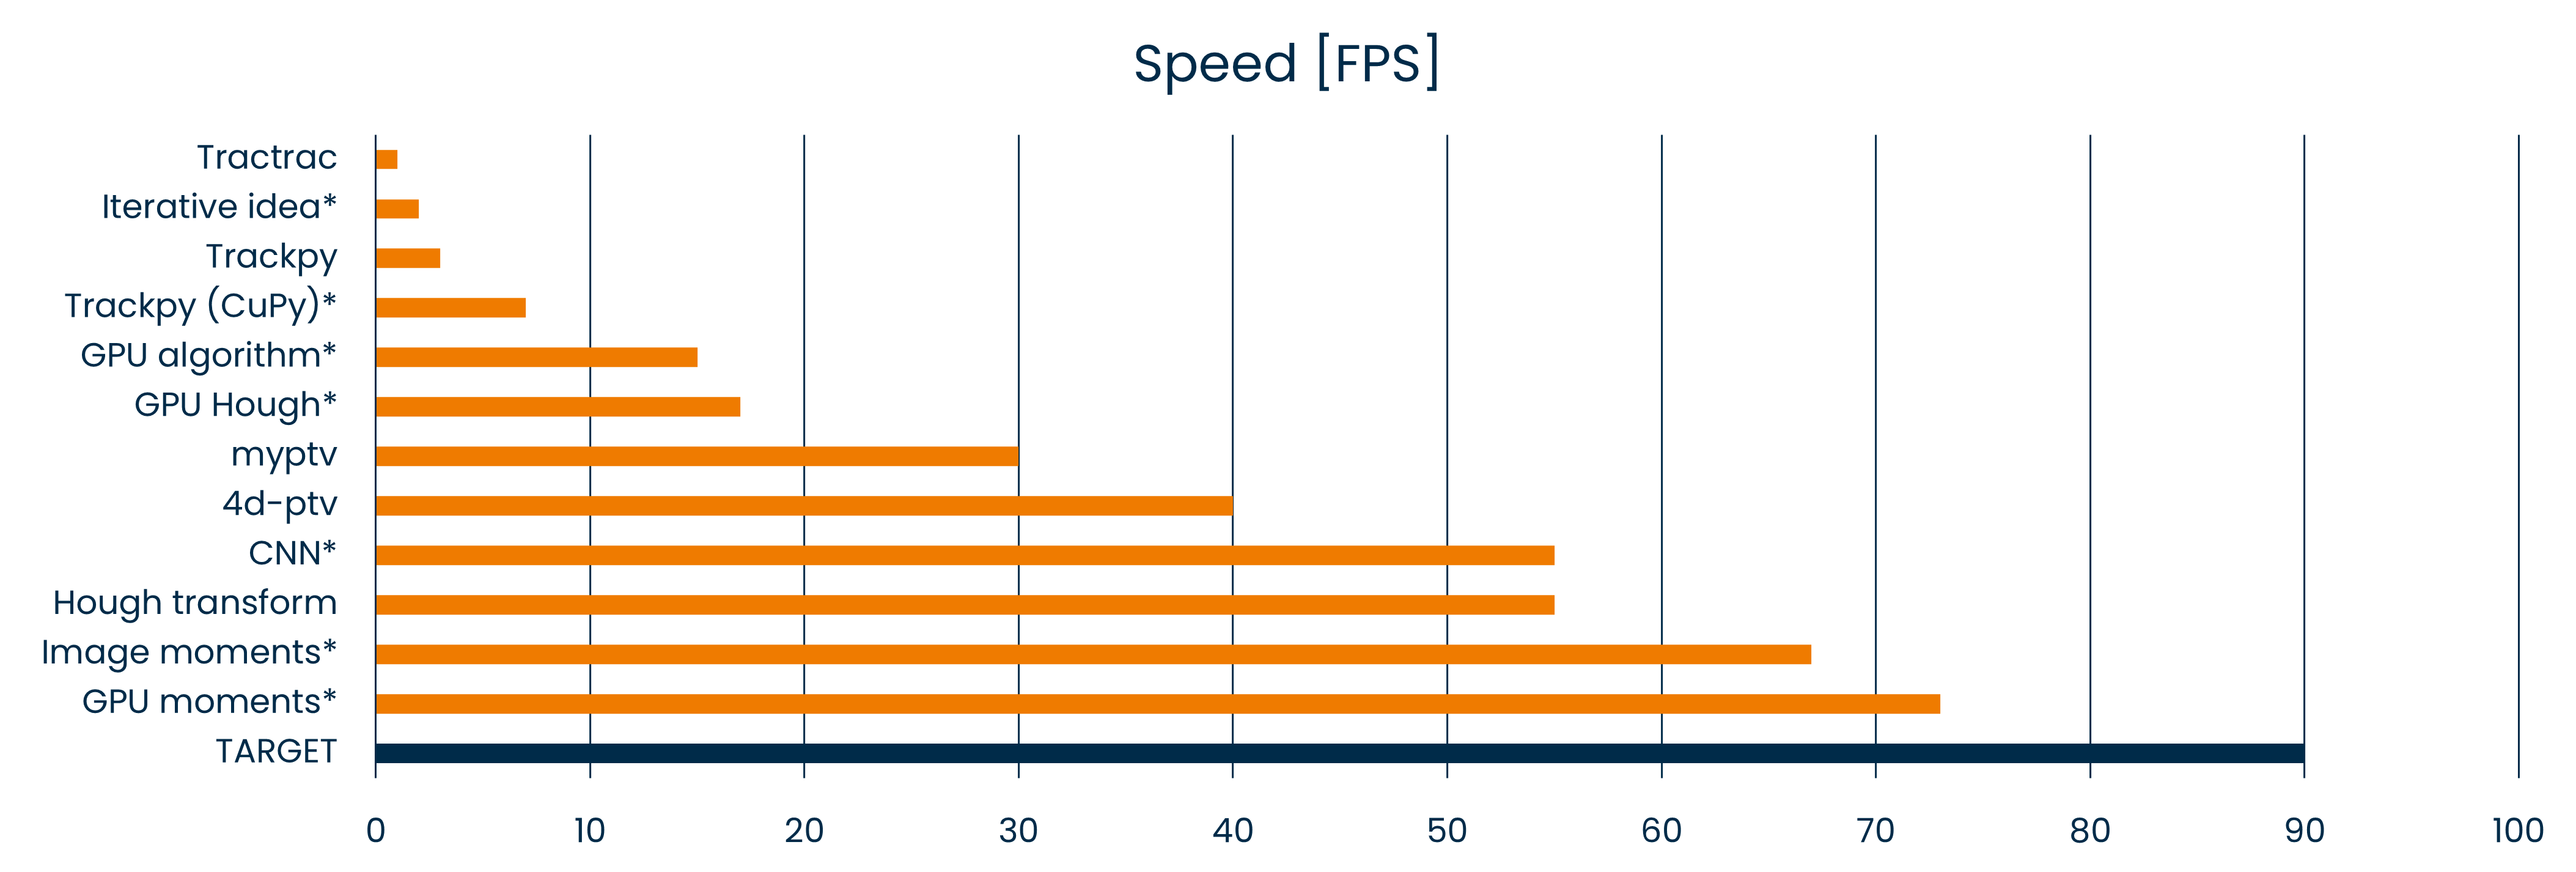
\includegraphics[width=\textwidth]{images/locate-speed-comparison.png}}
	\caption{\centering Performance evaluation of different approaches for the \textit{Locate} step.}
	%	\caption{\centering Comparing the speed of the Locate approaches. The ones marked with * are the ones developed by me.}
	\label{fig:intro:locate-speed}
\end{figure}
%Tutto più im poersonale
\summarysection{3D matching}

The \textit{3D matching} step is based on the stereoscopy technique, which matches pixels on different cameras to estimate the depth of a 3D point.
However, working on plain coordinates instead of textured images added the challenge of correctly matching bubbles across cameras.
For this step, no meaningful literature was found: several new algorithms were considered and compared in figure~\ref{fig:intro:3dmatching-cmp}.
The final choice was the best one among the algorithms whose speed was greater than the required 30 FPS.

\begin{figure}
	\centerline{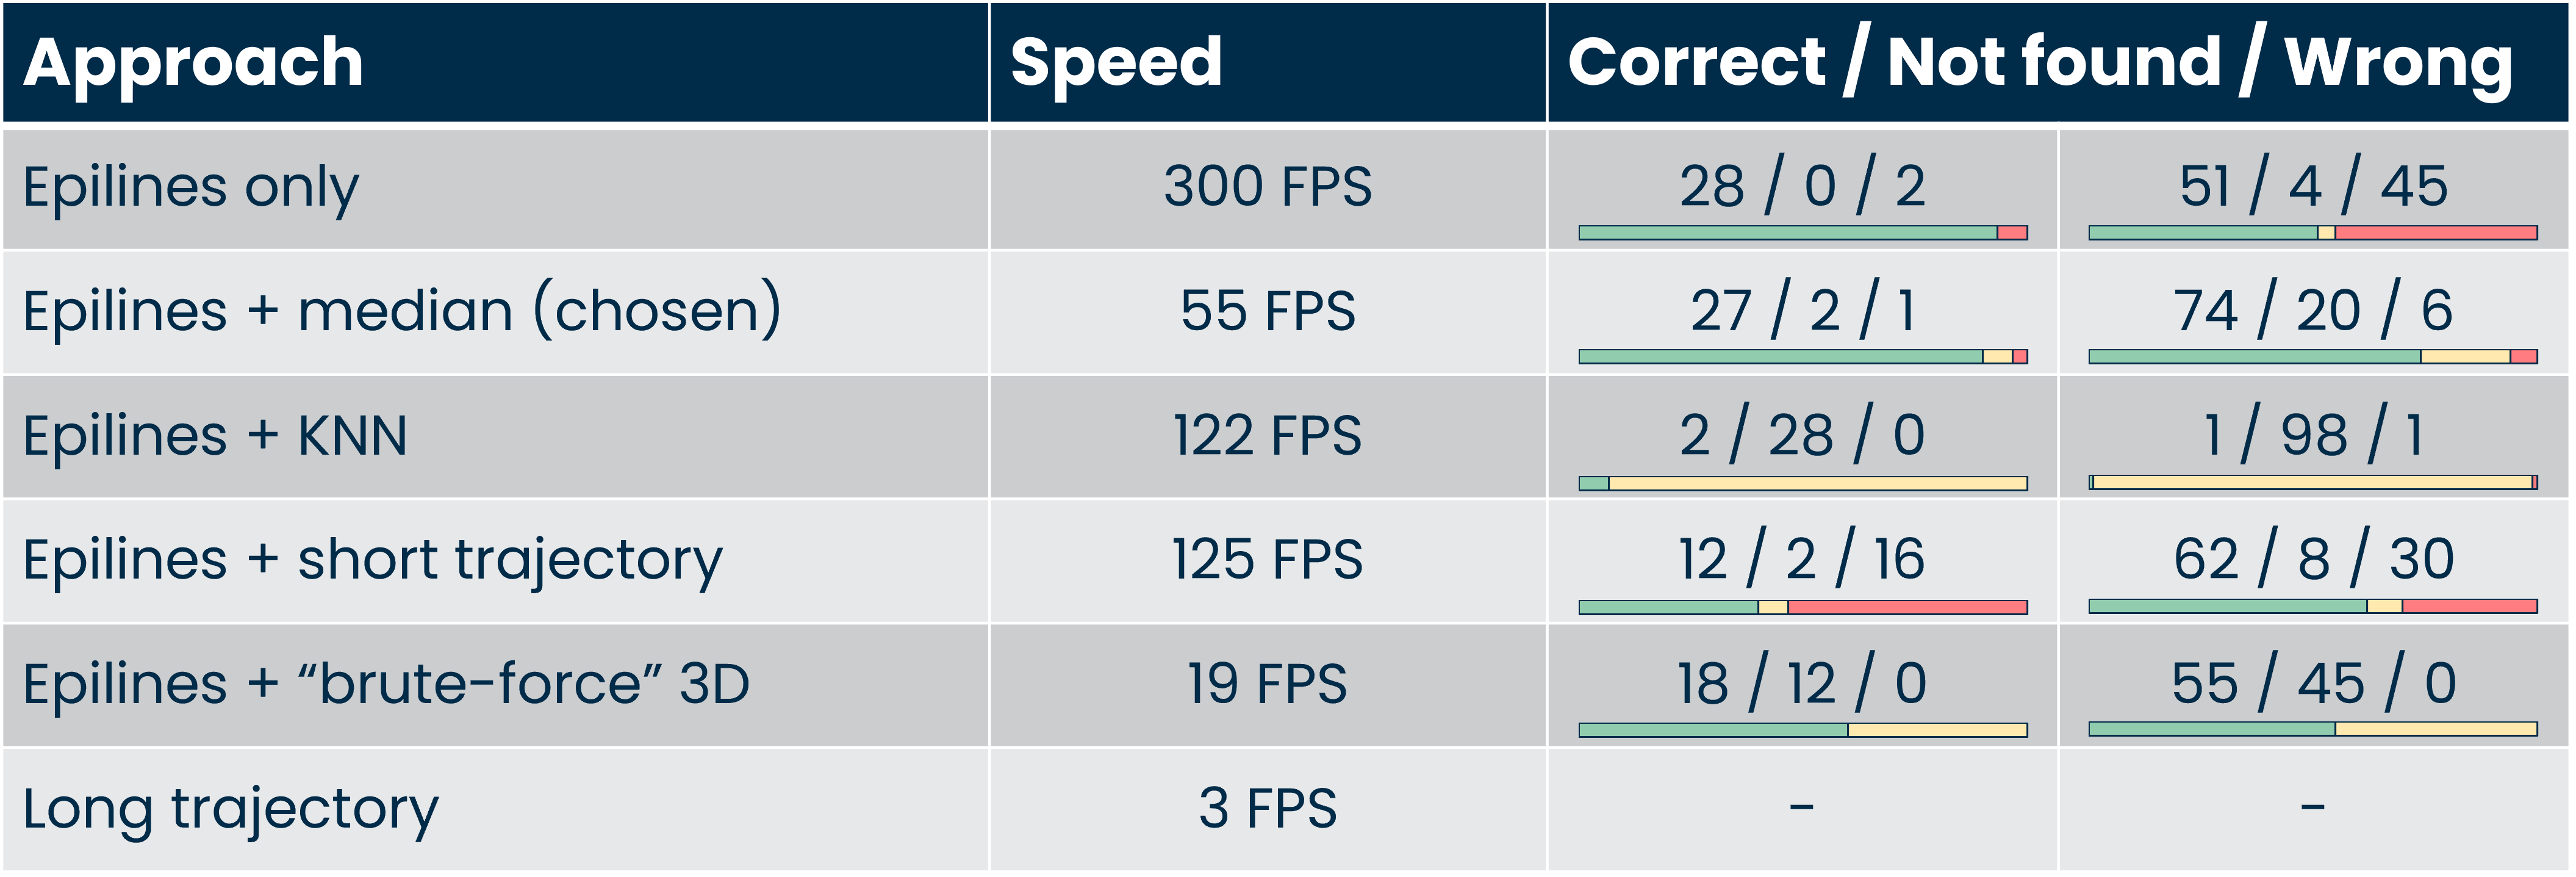
\includegraphics[width=0.9\textwidth]{images/3d-matching-comparison.png}}
	\caption{\centering Comparing speed and quality of the \textit{3D matching} approaches.}
	\label{fig:intro:3dmatching-cmp}
\end{figure}

\summarysection{Linking}

The \textit{Linking} step could be performed either in 2D, or in 3D.
While 2D \textit{link} was more popular in the literature, the results were not satisfactory in terms of accuracy.
As a consequence, a 3D \textit{linking} approach was chosen.
The final algorithm leverages the fact that the 3D bubbles are quite spaced out, to just link a bubble to the closest one in the next frame, provided that the distance is under a reasonability threshold.

\summarysection{Visualization}

Two different options were developed for the \textit{Visualization} step:
\begin{itemize}
	\itemsep 0em
	\item a simple, on-line rendering engine, built using the \texttt{Open3D} library. It is able to display the tracklets as soon as they are computed, but it is ephemeral and has little user control;
	\item a more advanced, off-line rendering engine, developed in the Unity game engine. It offers more control and freedom, but it requires that the reconstruction is complete and stored on disk.
\end{itemize}

\summarysection{Results}

When executed on a NVIDIA Jetson Orin Nano, the pipeline is able to process streams of 4 cameras at 38 FPS.
The results are excellent with scenes with up to 100 bubbles within the 3D space under observation.
The overall performance fully matches the objectives of this project.

While the speed is already higher than what was required, further optimizations may enable the pipeline to be executed on less powerful and cheaper hardware.
In this direction, figure~\ref{fig:intro:pipeline-usage} shows that the bottleneck is currently the \textit{Locate} step, which internally is mostly slowed by the loading of the frames to the RAM of the Jetson.
Optimizing this memory transfer would therefore enable the overall speed to improve.

% Results, such as an example the ones shown in figure~\ref{fig:intro:pipeline-usage}, shows several direction for future improvements. For instance, the bottleneck is the Locate step, mainly due to the transfer of each single captured frame to the RAM of the processing device, currently based on a NVIDIA Jetson Orin Nano.

% As shown in figure~\ref{fig:intro:pipeline-usage}, the bottleneck is the Locate step, mainly due to the transfer of each single captured frame to the RAM of the processing device, currently based on a NVIDIA Jetson Orin Nano.

Another interesting evolution of this work could be the improvement of the matching quality, to obtain an algorithm capable of analyzing setups with a more dense concentration of bubbles.
One of the possibilities to achieve this goal would be to find a better \textit{3D matching} algorithm, or to improve the speed of the \textit{Epilines + ``brute-force'' 3D} algorithm, which had a better quality, but was too slow.
Another direction to improve the \textit{3D matching} would be to have more information on the bubbles: for instance, if the bubbles were of different colors, the \textit{3D matching} step would just need to consider the subset of bubbles with similar color.

\begin{figure}
	\centerline{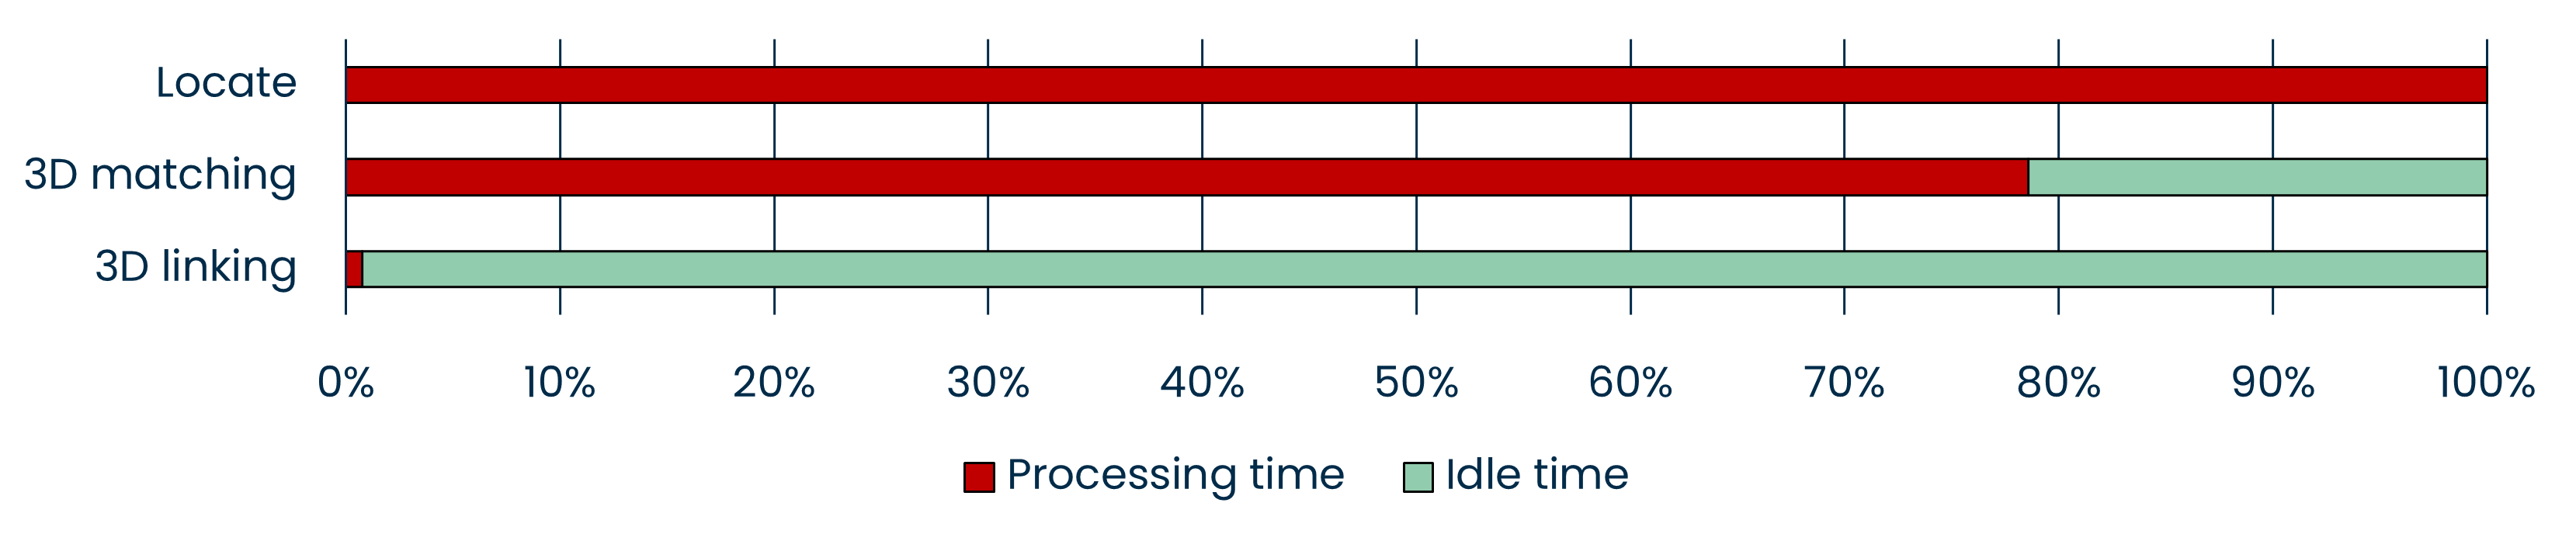
\includegraphics[width=0.9\textwidth]{images/pipeline-usage-graph.png}}
	\caption{\centering Time spent working and waiting for data, for each step of the pipeline: the bottleneck is the \textit{Locate} step.}
	\label{fig:intro:pipeline-usage}
\end{figure}
